%% Adaptado a partir de :
%%    abtex2-modelo-trabalho-academico.tex, v-1.9.2 laurocesar
%% para ser um modelo para os trabalhos no IFSP-SPO
\documentclass[
    % -- opções da classe memoir --
    12pt,               % tamanho da fonte
    openright,          % capítulos começam em pág ímpar (insere página vazia caso preciso)
    %twoside,            % para impressão em verso e anverso. Oposto a oneside
    oneside,
    a4paper,            % tamanho do papel. 
    % -- opções da classe abntex2 --schwinn
    % Opções que não devem ser utilizadas na versão final do documento
    %draft,              % para compilar mais rápido, remover na versão final
    paginasA3,  % indica que vai utilizar paginas em A3 
    BIBLATEX,           % indica para utilizar BIBLATEX em vez do abntex2cite
    REFINDENT,          % não fica exatamente no formato da ABNT, mas melhora muito a formatação
                        % não utilizar REFINDENT na versão final
    MODELO,             % indica que é um documento modelo então precisa dos geradores de texto
    TODO,               % indica que deve apresentar lista de pendencias 
    % -- opções do pacote babel --
    english,            % idioma adicional para hifenização
    brazil              % o último idioma é o principal do documento
    ]{ifsp-spo-inf-cemi} % ajustar de acordo com o modelo desejado para o curso

% ---
% Informações de dados para CAPA e FOLHA DE ROSTO
% ---
\titulo{ADA - Atribuição de Aulas}

% Trabalho em Equipe
% ver também https://github.com/abntex/abntex2/wiki/FAQ#como-adicionar-mais-de-um-autor-ao-meu-projeto
\renewcommand{\imprimirautor}{
\begin{tabular}{lr}
ANA PAULA MOURA MESSIAS DE SOUZA & SP3044505 \\
GUSTAVO SANTOS COSTA SOARES & SP3044491 \\
HENRIQUE LUIS BAESA & SP3045048 \\
ISABELLA VALERIO MAZARÁ & SP3045463 \\
JOSINEUDO DAS CHAGAS ARRUDA & SP3045439 \\
PAULO KENJI YOKOTA MUNEISCHI & SP3045382\\
\end{tabular}
}

\disciplina{PDS - Prática para Desenvolvimento de Sistemas}

\preambulo{Projeto apresentado no quarto ano do curso de informática integrado ao ensino médio, do Instituto Federal de Educação, Ciência e Tecnologia de São Paulo - Câmpus São Paulo, para a conclusão da disciplina de Projeto de Desenvolvimento de Sistemas.}

\data{2023}

\renewcommand{\orientadorname}{Professor:}
\orientador{GUSTAVO FORTUNATO PUGA}
\renewcommand{\coorientadorname}{Professor:}
\coorientador{LEONARDO ANDRADE MOTTA DE LIMA}

% ---
% informações do PDF
\makeatletter
\hypersetup{
        %pagebackref=true,
        pdftitle={\@title}, 
        pdfauthor={\@author},
        pdfsubject={\imprimirpreambulo},
        pdfcreator={LaTeX with abnTeX2 using IFSP model},
        pdfkeywords={abnt}{latex}{abntex}{abntex2}{IFSP}{\ifspprefixo}{trabalho acadêmico}, 
        colorlinks=true,            % false: boxed links; true: colored links
        linkcolor=blue,             % color of internal links
        citecolor=blue,             % color of links to bibliography
        filecolor=magenta,              % color of file links
        urlcolor=blue,
        bookmarksdepth=4
}
\makeatother
% --- 

% carregando aqui referencias quando utilizando BIBLATEX
\IfPackageLoaded{biblatex}{%
\addbibresource{referencias.bib}
\addbibresource{exemplos/abntex2-doc-abnt-6023.bib}
}{}

% ----
% Início do documento
% ----
\begin{document}


% Retira espaço extra obsoleto entre as frases.
\frenchspacing 

% ----------------------------------------------------------
% ELEMENTOS PRÉ-TEXTUAIS
% ----------------------------------------------------------
\pretextual

% ---
% Capa
% ---
\imprimircapa

% ---
% Folha de rosto
% (o * indica que haverá a ficha bibliográfica)
% ---
\imprimirfolhaderosto
%\imprimirfolhaderosto*
% ---

% Quando registrado na biblioteca
%\input{pre-fichacatalografica}

%Obrigatório para trabalhos com bancas oficiais
%\input{pre-aprovacao}


% -- resumo obrigatório
% ---
% RESUMOS
% ---

% resumo em português
\setlength{\absparsep}{18pt} % ajusta o espaçamento dos parágrafos do resumo
\begin{resumo}

Esse projeto, \ac{ada}, como o próprio nome sugere, fornece a coordenação e a execução do processo de atribuição de aulas aos docentes, no \ac{ifsp} - Câmpus São Paulo. Como objetivo, visa automatizar o processo atual, no \gls{excel}, de forma a tornar o preenchimento e a leitura dos dados do \ac{fpa} funcional e descomplicado. Destinado a cumprir a necessidade final dos docentes, o projeto igualmente será administrado por outros funcionários, cujos cargos estarão responsáveis pela atribuição naquele ano. Para executar todos os processos, no \gls{backend} será utilizado o \textit{\gls{framework}} open source \gls{springboot}, à linguagem Java, e no \gls{frontend}, o \textit{\gls{framework}} open source \gls{angular}, com base na linguagem TypeScript, e detalhes implementados através do Cascading Style Sheets $3^r^d$ version (\ac{css3}). Isso usando do \ac{sgbd} MySQL.

 \textbf{Palavras-chaves}: Atribuição. Aulas. Automatização. Docentes. Processo. Implementação.
\end{resumo}

% resumo em inglês
\begin{resumo}[Abstract]
 \begin{otherlanguage*}{english}

This project, Assignment of Classes (\ac{ada}), as its name suggests, coordinates and executes the process of assigning classes to professors at the Federal Institute of Education, Science, and Technology of São Paulo (\ac{ifsp}) - São Paulo Campus. As an objective, it aims to automate the current process, in \gls{excel}, to make filling and reading the data of the Activity Preference Form (\ac{fpa}) functional and uncomplicated. Destined to fulfill the final need of the professors, the project will also be managed by other employees, whose positions will be responsible for the attribution that year. To execute all the processes, in the \gls{backend}, the open-source \gls{springboot} \textit{\gls{framework}} will be used in the Java language, and the \gls{frontend}, the open-source \textit{\gls{framework}} \gls{angular}, based on the \gls{typescript} language, and details implemented through the Cascading Style Sheets $3^r^d$ version (\ac{css3}). This is using the MySQL Database Management System (\ac{sgbd}).
   \vspace{\onelineskip}
   \noindent 
   
   \textbf{Keywords}: Assignment. Classes. Automation. Teachers. Process. Implementation.
 \end{otherlanguage*}
\end{resumo}


\pdfbookmark[0]{\listfigurename}{lof}
\listoffigures*
\cleardoublepage
% ---

% ---
% inserir lista de abreviaturas e siglas
% ATENCAO o SHARELATEX/OVERLEAF GERA O GLOSSARIO SOMENTE UMA VEZ
% CASO SEJA FEITA ALGUMA ALTERAÇÃO NA LISTA DE SIGLAS É NECESSARIO UTILIZAR A OPÇÃO :
% "Clear Cached Files" DISPONIVEL NA VISUALIZAÇÃO DOS LOGS 
% ---
% https://www.sharelatex.com/learn/Glossaries

\ifdef{\printnoidxglossary}{
    \printnoidxglossary[type=\acronymtype,title=Lista de abreviaturas e siglas,style=siglas]
    \cleardoublepage
}{}


% ---
% inserir o sumario
% ---
\pdfbookmark[0]{\contentsname}{toc}
\tableofcontents*
\cleardoublepage
% ---


% ----------------------------------------------------------
% ELEMENTOS TEXTUAIS
% ----------------------------------------------------------
\textual

% ----------------------------------------------------------
% Introdução
% ----------------------------------------------------------
\chapter[Introdução]{Introdução}

No \ac{ifsp} Câmpus São Paulo, são mais de 350 docentes, com 56 na área de \ac{dit}. Logo, é essa a quantidade que participa da atribuição de aulas semestral e/ou anual, indicando seu extenso e intrincado processo. Além da referida quantidade, o que dá essas características à atribuição são os critérios a serem seguidos, desde a ordem de prioridade dos docentes até as preferências colocadas por cada um no \ac{fpa} e os regramentos presentes na resolução vigente – em 2023, ainda rege a Resolução n°109/2015, de 4 de novembro de 2015. 

Todo esse processo é realizado manualmente, através da entrega do \ac{fpa}, da ferramenta \gls{excel} e da comunicação particular constante entre o administrador daquele ano e o docente, principalmente no caso de \glspl{permuta}. Assim, procedem adversidades, conflitos interpessoais e atrasos, relatados semestralmente pelos docentes, principalmente pelos que ficam no final da fila de prioridade (os substitutos), e comentados, após contato da equipe, pelo administrador das atribuições da \ac{dit} atual, Evandro ..., e antigo, Leonardo Motta, os quais enfatizaram sobre a consequente sobrecarga em suas funções, ao tentar equilibrar a vontade de todos e, ao mesmo tempo, cumprir com a lei. 

Em decorrência disso, surge a necessidade da automatização de parte dos processos, que tem como objetivo a aprimoração do andamento do fluxo de trabalho \cite{sydle_2023}, trazendo como resultado o aumento da produtividade e a redução de custos e de erros \cite{totvs_2022}.

E, à vista do que foi exposto, o projeto retratado propõe a elaboração de um sistema que automatize os principais processos da atribuição - as seleções do \ac{fpa} e a \gls{permutação} - e, simultaneamente, cumpra o exigido na Resolução, e nos outros critérios estabelecidos hoje (como a prioridade da escolha do docente na atribuição) e que podem ser posteriormente adicionados. Esse sistema é o \ac{ada}.


\section{Objetivo}

O \ac{ada} visa apresentar uma solução e uma aprimoração às problemáticas da atribuição de aulas. Logo, oferecer um sistema Web responsivo de Single Application Page (\ac{spa}) aos funcionários, que automatize essa atribuição e a respectiva e consecutiva \gls{permutação} (caso habilitada), sem a necessidade de organização manual e de negociações individuais e extraoficiais. 

Com processos correspondentes aos problemas centrais, terá a implementação do \gls{login}, pelo e-mail oficial do Instituto no Google, tratando do gerenciamento geral dos docentes e dos administradores; da automatização do \ac{fpa}, tratando da dificuldade de estruturação da grade horária seguindo todos os critérios e os regramentos; e da automatização das negociações à \gls{permuta}, tratando dos atritos e da dificuldade de comunicação gerados.

Consequentemente, o sistema proporcionará, a princípio, um ambiente em que o administrador superior e os subadministradores consigam controlar e ordenar os critérios às suas área e subáreas, respectivamente, e habilitar funções como a \gls{permutação} e a desativação de um  em determinada matéria. Ademais, proporcionará um ambiente em que o docente consiga selecionar todas as suas preferências e solicitar suas \glspl{permuta}(caso habilitadas) em um único local, sem demasiadas complicações e processos. 

Uma operação antes com responsabilidades individuais e organização manual, a qual incorre de mais erros devido a subjetividade e os problemas humanos, passará a ser uma operação tecnológica mais limpa e funcional, com menos erros.

\section{Análise de concorrentes}

A Análise de Concorrência é valiosa para obter conhecimento sobre como outros sistemas – com o mesmo propósito ou um próximo – desenvolvem seu projeto, implementam seus processos, atraem clientes, apresentam sua plataforma, gerenciam seus dados, fecham parcerias, entre outros; fatores importantes a serem considerados tanto para o aprimoramento do sistema que você está realizando, quanto para saber com quem está disputando o mercado. 

Nessa pesquisa, a equipe achou algumas concorrências referentes ao processo de atribuição de aulas. Entre elas, vale a pena serem citadas a \ac{sed} e o \ac{sig} .
A \ac{sed} apresenta um sistema que abrange toda a rede educacional estadual de São Paulo (SP) \cite{secretaria_sp}. Através dele, o docente pode manifestar seu interesse em aulas vagas e livres ou em substituição das escolas, pela pesquisa por uma escola específica ou uma disciplina. Quanto à prioridade de escolha, o docente pode alterar a ordem da sua seleção de acordo com as escolas em que prefere lecionar. 

E o \ac{sig} \cite{sig} aparenta apresentar um sistema parecido, onde o docente preenche e envia a inscrição e o requerimento de ampliação de carga horária de forma digital. Entretanto, as informações são escassas, baseadas na página de divulgação da \ac{urh} \cite{urh}, onde está o sistema; o tutorial leva a uma página de erro. Contudo, uma diferença fundamental é o fato de ser voltado apenas às \ac{etecs}.

Com o conhecimento adquirido foi possível observar pontos a serem implementados no \ac{ada}, como a disponibilidade de um tutorial no início e mensagens de ajuda ao longo da página – além do ótimo design da \ac{sed} que pode servir de inspiração. E pontos semelhantes foram justamente essa escolha de aulas pelo docente, de acordo com sua subárea, e o \textit{login} que não permite o cadastro de pessoas não autorizadas (um usa do \ac{cpf} e o outro do e-mail).

Todavia, foi igualmente possível observar a necessidade do sistema apresentado neste projeto, que prevê erros retratados nos concorrentes, como o atraso considerável do primeiro devido às longas filas de seleção, a ausência de verificação de componente curricular, abrindo uma brecha para qualquer docente lecionar a disciplina sem ter o nível de escolaridade necessária, e os erros no processo de pontuação para prioridade de escolha – retratados em uma matéria \cite{g1_2020} da \gls{globo} e relatados pela Inês Paz, coordenadora da subsede da \ac{apeoesp} e vereadora de Mogi, \cite{acioli_2021}: “A classificação saiu com muitos erros e os professores não estão tendo um retorno às suas perguntas, enquanto isso, a atribuição continua acontecendo com esses profissionais correndo o risco de se prejudicarem”. Já do segundo concorrente, a falta de tutorial e dificuldade na compreensão da página de \textit{login}. 

À vista do citado acima, o sistema \ac{ada} subsidia uma série de ações que permitem o cruzamento de dados e processos que diferenciam a ideia de qualquer outra anterior; e, por ser voltado ao Instituto em específico, igualmente permite uma melhor análise dos \glspl{feedback} e tratamento dos erros. Portanto, será implementado de forma a considerar boas práticas de concorrentes e aplicações parecidas, e, principalmente, dificuldades nelas encontradas, não atendo-se a um ciclo de falhas.

%\input{textos-revisao-literatura}

%---------------------------------------------------------------------------------------
\chapter{Ideia}

A fim de implementar um sistema que trate dos problemas citados e consiga atingir os objetivos propostos, são necessários processos e a utilização de determinadas tecnologias, citadas no subtópico . 

Os processos principais são três, o cadastramento dos usuários, a automatização do \ac{fpa} e a possibilidade de habilitação de outros processos, por parte dos administradores, com destaque à permutação dos horários já atribuídos e à desativação de um docente em determinada matéria.

\section{Cadastramento dos usuários}

Preliminar à qualquer utilização do \ac{ada}, o Administrador Superior (\gls{superAdmin}), será cadastrado pelos próprios programadores e terá o maior nível de acesso, podendo realizar quaisquer alterações e controlar quais serão os Administradores (\gls{admin}). 

Então, os outros funcionários receberão um link para acessarem o \ac{ada} via Google, pelo e-mail institucional - o que evita acessos não permitidos, e serão atribuídos instantaneamente ao papel de Professor (\gls{professor}); como mencionado, a mudança desse nível de acesso para o de \gls{admin} é realizada pelo \gls{superAdmin}. E acessos posteriores poderão ser através do Google ou do prontuário e senha.

\subsection{Configuração do ambiente}

A configuração do ambiente é um subprocesso, em que o \gls{superAdmin} será responsável por habilitar a possibilidade de \glspl{permuta} e de desativação do docente em uma disciplina; prazos limites à organização; e definição ou atualização dos critérios da atribuição - baseados na legislação vigente e na ordem de prioridade de escolha das disciplinas.

E o \gls{admin} será responsável pela subárea, consequentemente, por subir a grade horária; determinar prazos específicos; autorizar a \gls{permutação} e se deseja participar da aprovação das \glspl{permuta}; controlar os docentes desativados; e adicionar\footnote{Essa adição será manual e de acordo com a prioridade escolhida. Portanto, um subprocesso, onde o \gls{admin} colocará os docentes na ordem e, igualmente, poderá alterá-la em caso de erro ou modificações futuras.} os que participarão de sua subárea. 


\begin{figure}[h]
    \centering
    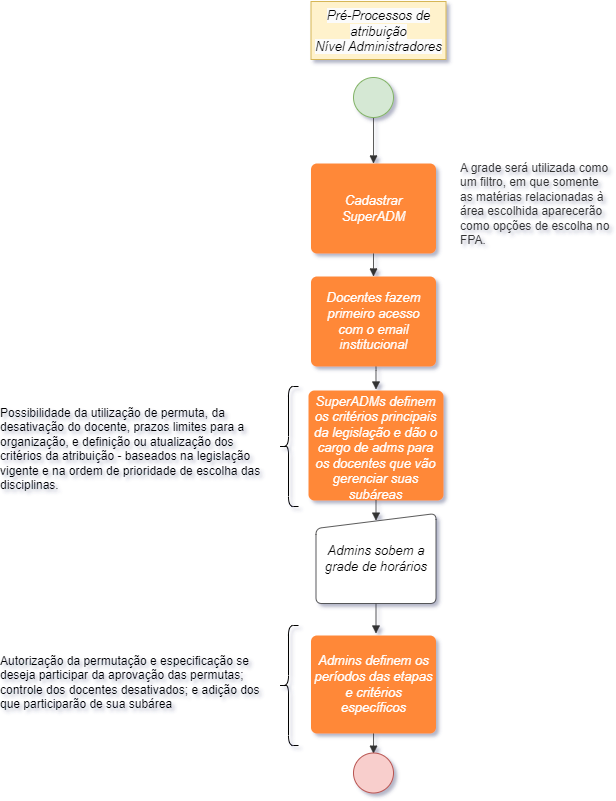
\includegraphics[width=0.85\textwidth]{anexos/Fluxograma/FluxogramaCadastramento.png}
    \caption{Fluxograma dos pré-processos de atribuição}
    \label{fig:figura1} 
\end{figure}

\section{Automatização do FPA}

Finalizada a organização do sistema pelos administradores e todos os docentes cadastrados nas subáreas, eles poderão acessar o sistema e iniciar o processo de escolha da disponibilidade de horários e da preferência de aulas (prioritária e secundária) e de atividades. Conforme é realizado esse processo, o ADA verifica se cada escolha segue os regramentos, e impossibilita a escolha de disciplinas em conflito; igualmente, informa com uma mensagem breve caso o docente selecione uma em que foi desativado. 

\begin{figure}[t]
    \centering
    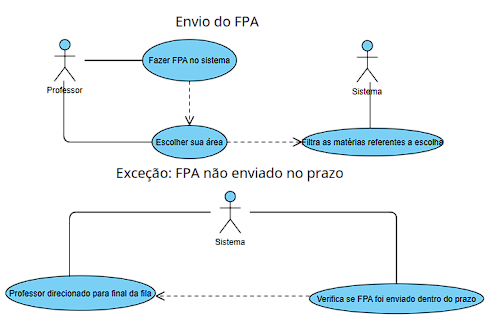
\includegraphics[width=0.7\textwidth]{anexos/CasosDeUso/CasoDeUso_EnvioFPA.png}
    \caption{Caso de uso do envio de preferências}
    \label{fig:figura2} 
\end{figure}

A determinação da preferência de atividades poderá ser modificada dentro do prazo de entrega estabelecido pelo \gls{admin}. Porém, ao encerrar o prazo, o \ac{ada} percorre a lista de docentes, em ordem decrescente, e atribui as aulas de acordo com o selecionado. O processo é interrompido - e é armazenado o que já foi feito - caso haja conflito com uma disciplina já escolhida; assim, aquele docente receberá uma solicitação para alterar sua escolha dentro de determinado prazo.

\begin{figure}[h]
    \centering
    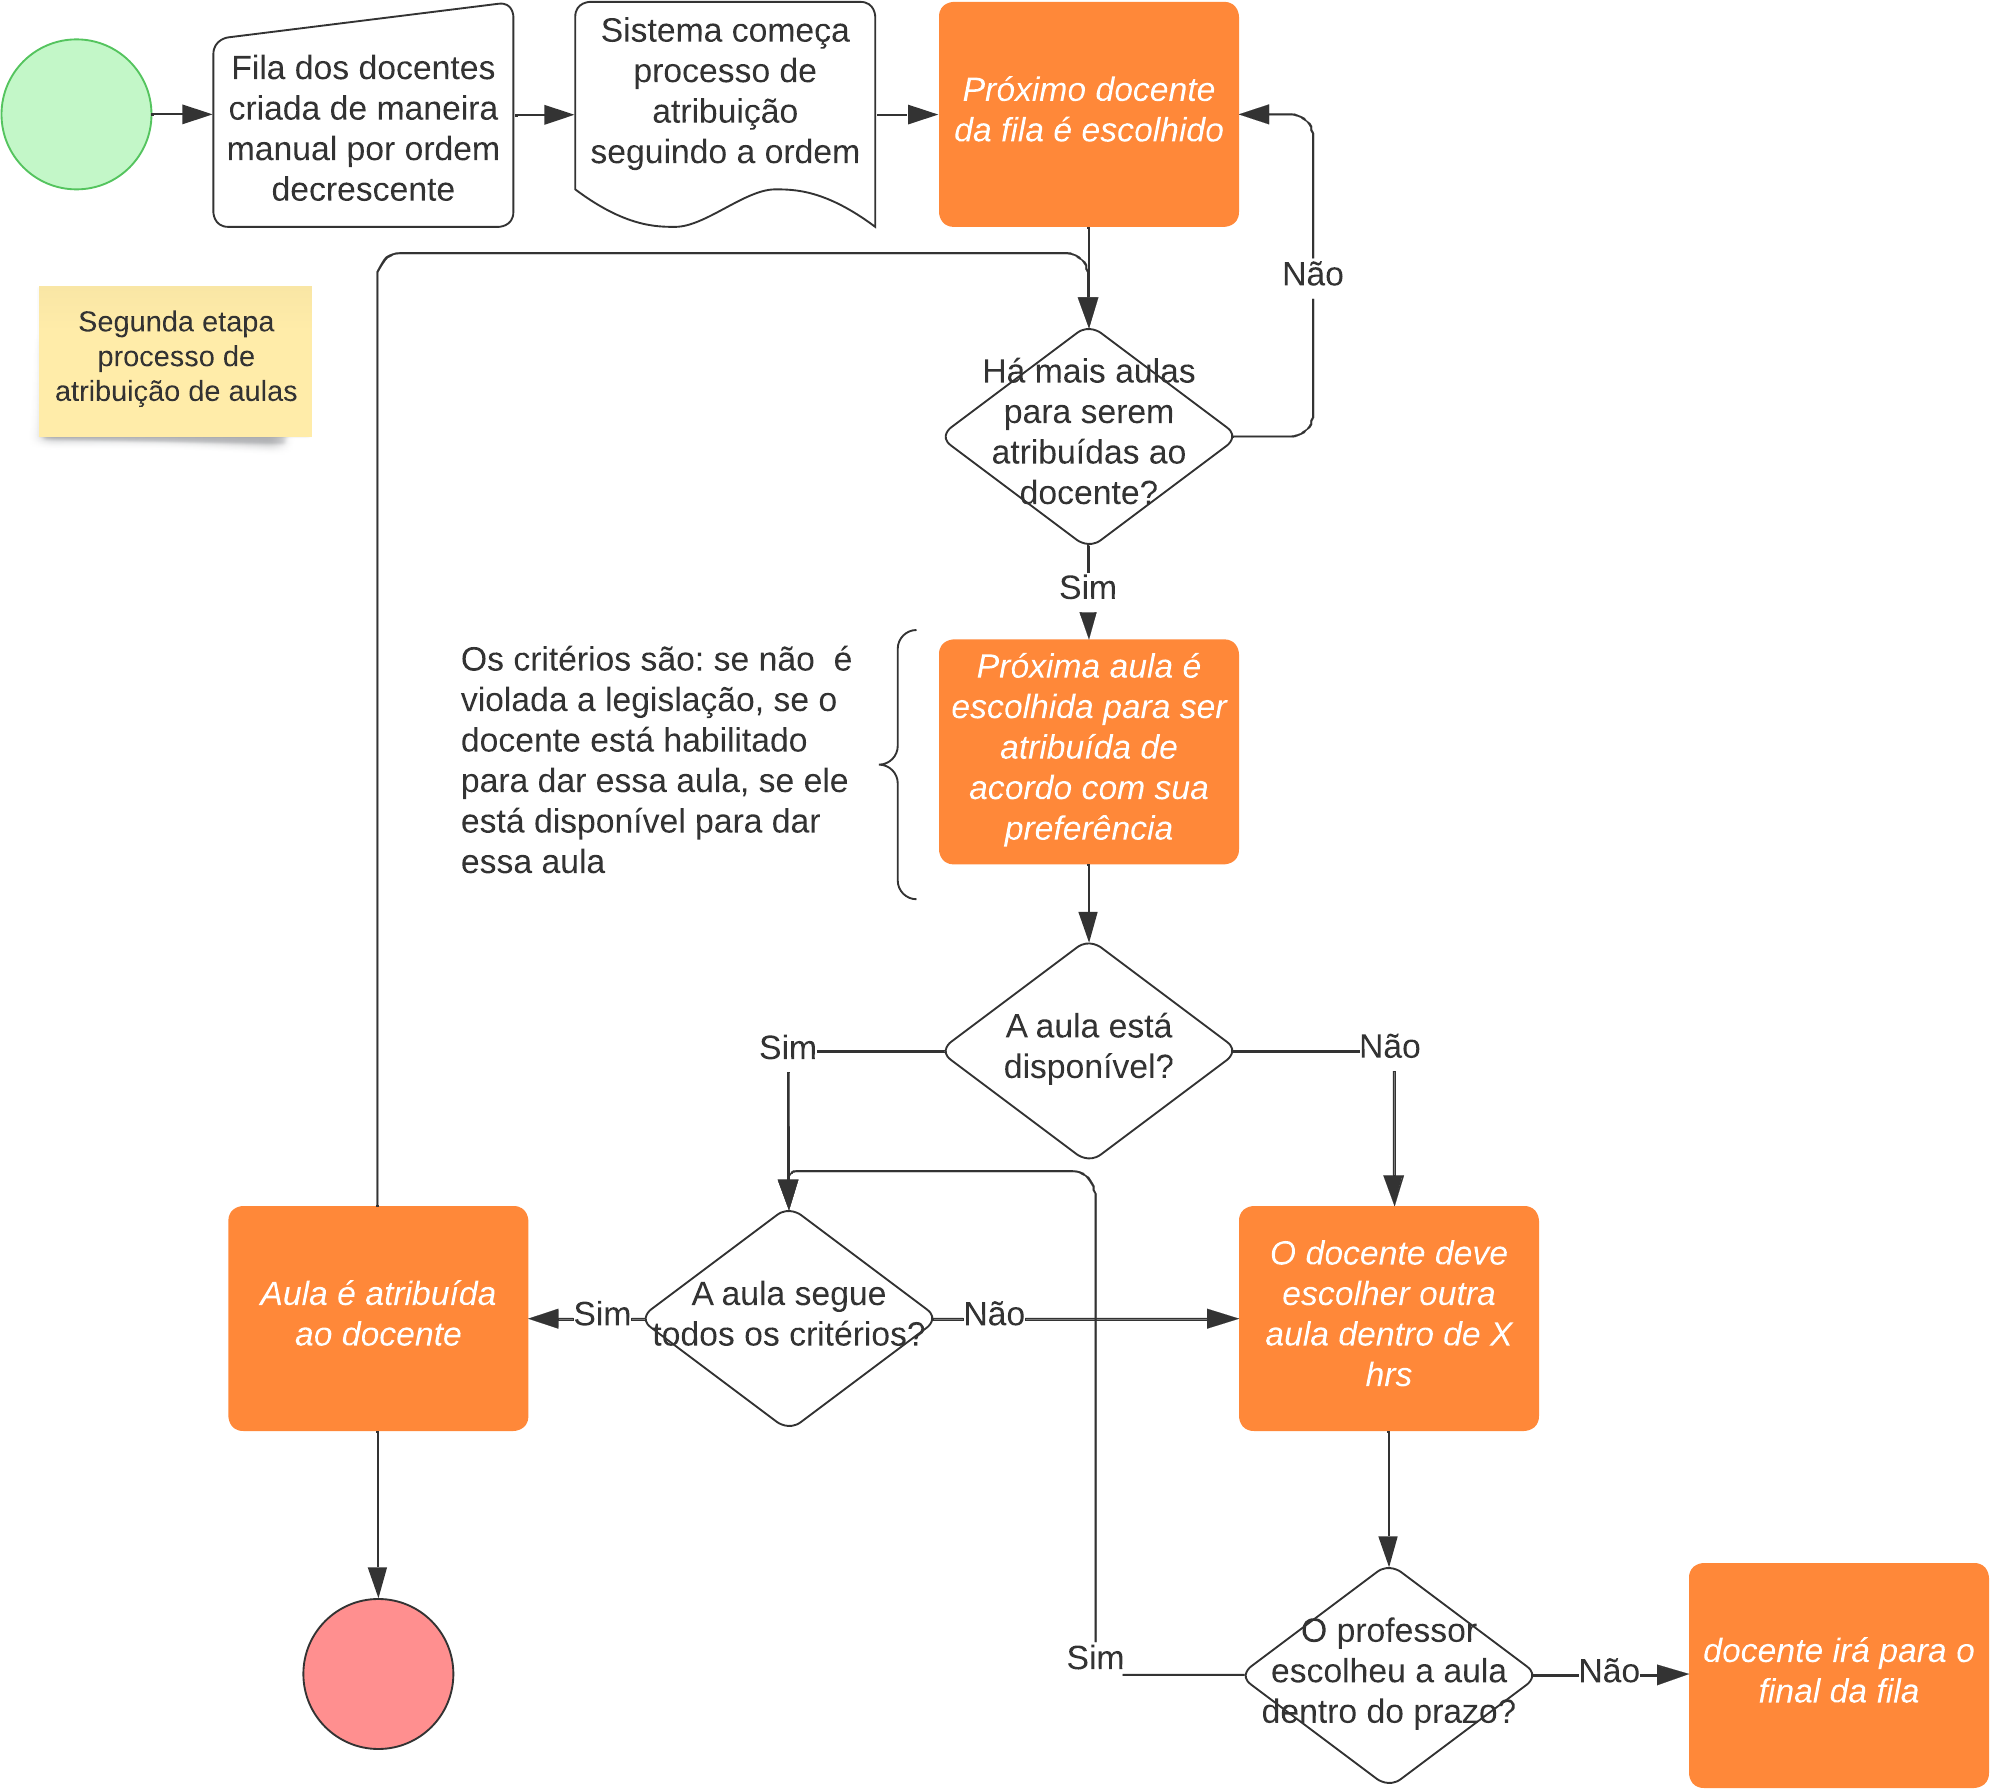
\includegraphics[width=0.7\textwidth]{anexos/Fluxograma/FluxogramaProcessoAtribuicaoAulas.png}
    \caption{Fluxograma da atribuição de aulas}
    \label{fig:figura3}
\end{figure}

\section{Permutação}

A permutação é aberta, caso habilitada com a conclusão da grade pelo sistema. De modo geral, é feita com a solicitação de um docente pela troca de sua aula por uma específica do outro, selecionada na grade. É impossibilitada mais de uma solicitação, ao mesmo tempo, para uma mesma aula; Apenas é liberada quando essa for aceita ou recusada. Igualmente é impossibilidada a solicitação de alguma que descumpra o regramento. 
Caso o \gls{admin} seja moderador, ele terá que aprovar a aceitação da permuta pelo segundo docente.


Por fim, é gerada a grade horária final, onde os docentes e os administradores conseguem visualizar e salvar a atribuição de aulas da subárea. Além da possibilidade de gerar o \ac{fpa} com essa grade pronta.

\begin{figure}[h]
    \centering
    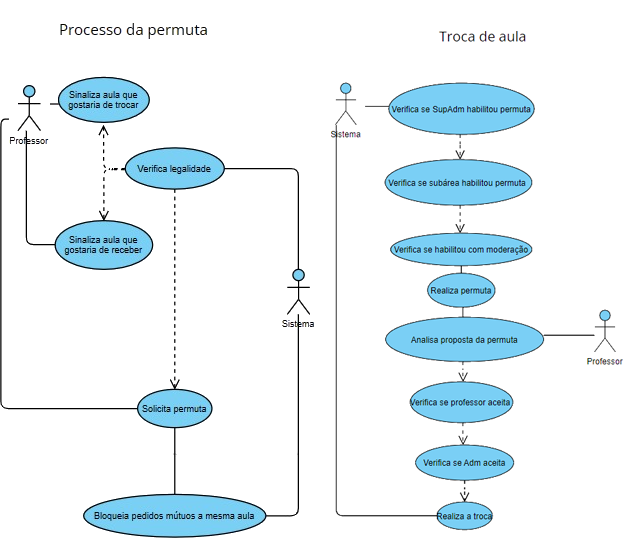
\includegraphics[width=1\textwidth]{anexos/CasosDeUso/CasoDeUso_ProcessoPermutaFULL.png}
    \caption{Caso de uso troca de Aula}
    \label{fig:figura4} 
\end{figure}

\section{Tecnologias e ferramentas aplicadas}

Em vista do desenvolvimento do \ac{ada} de maneira concisa e eficaz, a implementação de tecnologias e suas respectivas ferramentas se faz necessária. Além disso, repositórios de controle de versão e Integrated Development Environment (\ac{ide}) deverão, e serão, utilizados.

\subsection{Tecnologias}
A seguir estão as tecnologias utilizadas, suas características principais e, assim, porque foram escolhidas. A finalidade principal desse conjunto é escrever a aplicação de forma rápida e eficiente, concentrando toda a energia no desenvolvimento e aplicação da lógica, e, logo, poupando tempo em funcionalidades básicas.

\subsubsection{Django}
É um \gls{framework} \textit{web} \textit{\gls{open source}} e de alto nível, desenvolvido em Python, que se baseia no padrão \ac{mtv}, apresentando semelhança com o \ac{mvc}. Assim, segue o princípio \ac{dry}\footnote{Permite que as aplicações sejam desenvolvidas com a maior quantidade de aproveitamento de código possível.}, é moderadamente opinativo \footnote{Flexibilidade que o \gls{framework} dá aos desenvolvedores à resolução dos problemas. Opinativo, já possui uma maneira correta de resolvê-los, sem margens; não-opinativo, não possui essas regras e deixa livre para resolvê-los como quiser. Django equilíbrio entre soluções prontas e arquitetura desacoplada com liberdade na resolução de erros. }e apresenta suporte para erros comuns de segurança. Além desses benefícios, foi escolhido devido a sua aplicação em grandes empresas (como \gls{mozilla} e \gls{pinterest}) e, principalmente, no \ac{suap} do \ac{ifsp}, o que permite manter o padrão de tecnologias no Instituto.
\cite{lucas_2021} \cite{andrade_2019}

\paragraph{\ac{mtv}}
Derivação da arquitetura de software \ac{mvc}, de três camadas, altera a nomenclatura e a relação entre os arquivos. O Model permanece o mesmo, como um canal de conexão entre os tipos de dados e como serão armazenados no Banco de Dados, e a exibição ao ter requisição à View. Essa é responsável, então, pelo gerenciamento das requisições e a lógica de negócio, com a formatação dos dados enviados pelo Model. Por fim, o Template é a interação com o usuário, através de uma exibição estática ou inserção de sintaxe de conteúdo dinâmico, com a renderização dos dados entregues pela View.
\cite{silva_2020}
\
\subsubsection{Python}
É uma linguagem de programação \textit{\gls{open source}} e de alto nível, interpretada em scripts e orientada a objetos, que apresenta tipagem dinâmica\footnote{Tipo do dado é determinado no tempo de execução, de acordo com o valor do dado, não a partir da sua variável.} forte. Logo, prioriza a agilidade por meio de sua fácil compreensão, sintaxe menor e simplificada, sem muitas exigências gramaticais. E é por isso que foi escolhida, uma ótima opção que supriu de forma excelente a necessidade de uma aprendizagem rápida e fácil codificação nos dispositivos do \ac{ifsp}, além de poder ser facilmente integrada a outras linguagens de programação populares, caso seja necessário no decorrer do projeto.
\cite{amazon_2023} \cite{melo_2021}

\subsubsection{AJAX}
O \ac{ajax} é uma técnica de desenvolvimento \textit{web}, caracterizada pela criação de aplicações interativas através de requisições ao servidor. Uma junção das funcionalidades do \ac{js} com a troca dos dados, armazenados e transmitidos, nesse caso, pelo \ac{json} (mais próximo do \ac{js}). Foi escolhido justamente por servir como um canal de comunicação independente entre o cliente e o servidor.
\cite{andrei_2019} \cite{carvalho_2007}

\subsubsection{JavaScript}
É uma linguagem de programação de alto nível e interpretada em scripts, com recursos de \ac{oo} e \ac{api}, que apresenta tipagem dinâmica. Assim, por meio de um funcionamento assíncrono \footnote{A programação assíncrona é uma técnica na qual o programa inicia uma tarefa e ainda é capaz de executar simultaneamente outros eventos, ao invés de bloquear processos para esperar o término da execução.}, usa trechos dos códigos HTML para renderizar funções que proporcionem uma interação dinâmica local com o conteúdo da página. Foi escolhida para, em conjunto com o \ac{ajax}, proporcionar essa dinamicidade em tempo real, recarregamento automático.
\cite{mozilla_2023} \cite{melo_2021}

\subsubsection{HTML}
O \ac{html} é uma estrutura responsável pela exibição dos dados no navegador \textit{web}, caracterizado por seus elementos hierarquizados e sua marcação que abriga elementos como tags. Na aplicação ADA, é utilizada nos templates, explicados no parágrafo 2.4.1.1.1 .
\cite{mozilla_2023b}

\subsubsection{CSS}
O \ac{css} é uma linguagem de marcação, responsável pela estilização de elementos \ac{html}. Foi escolhido a fim de ajudar na formatação dos templates em detalhes específicos que, por vezes, não são compreendidos pelo framework, pois esse é mais genérico.
\cite{totvs_2020}

\subsubsection{Bootstrap}
É um \gls{framework} \textit{front-end}, logo, voltado à estilização, e \textit{\gls{open source}}. Foi escolhido devido à agilidade no desenvolvimento da página para o usuário, característica pelos frameworks, e, principalmente, devido à responsividade proporcionada.
\cite{andrei_2019} \cite{lima_2021}

\subsubsection{SQLite3}
\ac{sgbd}, o SQLite é uma biblioteca em linguagem C, \textit{\gls{open source}}, acoplada ao banco de dados \ac{sql}. Escolhido porque entrega o banco em conjunto com a aplicação (é embutido), sem a necessidade de um servidor, já que optamos por realizar a arquitetura \ac{mtv} em vez de Cliente/Servidor.
\cite{silva_2007} \cite{carlos_2019}

 \subsection{Hospedagem}
 A fim de ter uma instância em nuvem e conseguir fazer a hospedagem do site, foi utilizada a \ac{aws}. É uma plataforma que disponibiliza diversos serviços de computação em uma rede de servidores remotos. Assim, é possível criar instâncias de máquinas com sistema operacional Windows ou Linux, de modo que a aplicação funcione constantemente, sem necessitar que um computador pessoal fique ligado. 

 Somente com ela já é disponibilizada a aplicação na \textit{web}. Todavia, o acesso é difícil, pois aparecerá somente o endereço IPv4 público da máquina virtual criada. Para resolvê-lo, foi comprado o domínio \url{https://mottarios.cloud/} no \textit{website} Hostinger.

 \subsection{Criptografia}
A criptografia, para fornecer uma aplicação segura, foi configurada seguindo o protocolo \ac{https}, 

De forma a verificar seu devido funcionamento, foi utilizada a certificadora \textit{Let’s Encrypt}. Assim, teve uma confirmação de que há controle sobre o domínio citado anteriormente, e, com isso, foi gerado um certificado \ac{ssl}/\ac{tls} para ele. Após adicionar o certificado, a aplicação atingiu nota A no \textit{SSL Labs}. Para mais informações: \url{https://www.ssllabs.com/ssltest/analyze.html?d=mottarios.cloud}
\
\begin{figure}[h]
    \centering
    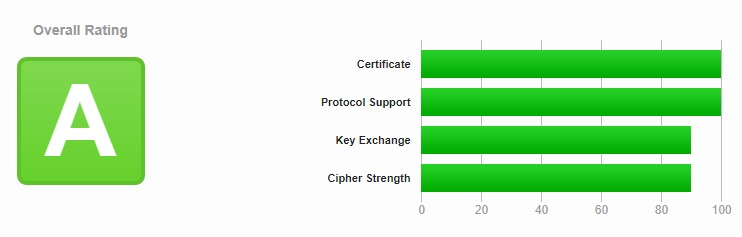
\includegraphics[width=1.00\textwidth]{anexos/DiagramaDeArquitetura/Certificado_NotaA.jpeg}
    \caption{Certificado SSL/TLS}
    \label{fig:figura1} 
\end{figure}

\subsection{Ferramentas}

\subsubsection{Controle de Versão}
É utilizado o \ac{svn}, uma ferramenta que armazena projetos e todas suas versões em um servidor centralizado. Escolhido devido à padronização dos projetos e devido à capacidade de armazená-los de forma segura. Igualmente, é utilizado o \gls{github}, de forma secundária, devido à familiaridade e à melhor organização, principalmente tratando-se do uso de \textit{branchs}.

\subsubsection{Documentação}
É utilizado o Overleaf, um editor e compilador \textit{online} de \gls{latex}. A fim de seguir a padronização dos projetos anteriores e para uma produção mais dinâmica dos documentos \gls{latex}, já que permite o compartilhamento dos arquivos entre outras pessoas e a edição simultânea. 

\subsubsection{Programação}
É utilizado o \ac{vscode}, um editor de código-fonte criado pela Microsoft. Foi escolhido devido a sua dinamicidade para codificação e a familiaridade que os membros da equipe já possuem com a ferramenta. 

Ademais, também é utilizado o codespace, que, por sua vez, é um ambiente de desenvolvimento hospedado em nuvem, promovido pela plataforma GitHub. Assim, é possível programar através do navegador, sem precisar de uma aplicação instalada na máquina, facilitando a programação no \ac{ifsp}. 

\subsection{Diagrama de Arquitetura}

\begin{figure}[h]
    \centering
    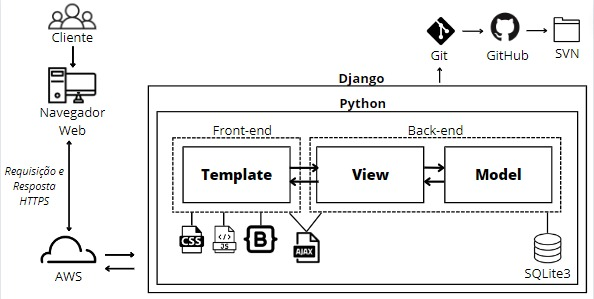
\includegraphics[width=0.96\textwidth]{anexos/DiagramaDeArquitetura/DiagramaDeArquitetura.jpeg}
    \caption{Diagrama de arquitetura}
    \label{fig:figura1} 
\end{figure}

%  LISTA
% \begin{itemize}
%   \item List entries start with the \verb|\item| command.
% \end{itemize}

%---------------------------------------------------------------------------------------







% ----------------------------------------------------------------------

\chapter{Links do projeto}

\section{Fluxograma}

\quad
\qrcode[height=2in]{https://drive.google.com/file/d/1xzoMxAUX7tdHU5OjtRSQ4jP6CebgEH7I/view?usp=sharing}
\quad
\href{https://drive.google.com/file/d/1xzoMxAUX7tdHU5OjtRSQ4jP6CebgEH7I/view?usp=sharing}{<Fluxograma>}

\section{Repositório GitHub}

\quad
\qrcode[height=2in]{https://github.com/mottariosifsp}
\quad
\href{https://github.com/mottariosifsp}{<https://github.com/mottariosifsp>}

\section{Repositório Subversion}

\quad
\qrcode[height=2in]{https://svn.spo.ifsp.edu.br/viewvc/A6PGP/A2023-PDS-QUA/Mottarios/}
\quad
\href{https://svn.spo.ifsp.edu.br/viewvc/A6PGP/A2023-PDS-QUA/Mottarios/}{<Repositório Subversion (SVN)>}

\section{Casos de Uso}

\quad
\qrcode[height=2in]{https://drive.google.com/file/d/1rqvJaLzmERWgdO2qMnBVHQN4HF3N7Qjs/view?usp=sharing}
\quad
\href{https://drive.google.com/file/d/1rqvJaLzmERWgdO2qMnBVHQN4HF3N7Qjs/view?usp=sharing}{<Casos de Uso>}

\section{Protótipo de Baixa Fidelidade}
\quad
\qrcode[height=2in]{https://drive.google.com/file/d/1XEk7EWKSioQtgcbZUR_zJ1KhJ9tyWydZ/view?usp=sharing}
\quad
\href{https://drive.google.com/file/d/1XEk7EWKSioQtgcbZUR_zJ1KhJ9tyWydZ/view?usp=sharing}{<Protótipo de Baixa Fidelidade>}

\chapter{Considerações Finais}
Por meio das questões e relatos expostos ao longo da pesquisa sobre o tema do projeto, ficou cada vez mais evidenciado o grande acréscimo e consequente aprimoramento que o \ac{ada} trará à \ac{dit}, do \ac{ifsp} Câmpus São Paulo; a aplicação é factível, promissora e necessária. 

Quanto às dificuldades na atribuição de aulas, são comuns e recorrentes, e o sistema é projetado visando facilitar essa operação. Porém, é um projeto que pode ser expandido tanto para outras áreas quanto para outros Câmpus ou, inclusive, outras Instituições de Ensino, o que significa um grande potencial atual e, também, futuro do sistema.

Isso graças ao desenvolvimento melhor estruturado, que abriga todas as nuances dos processos e seus respectivos planos de ação, proporcionado pelas reuniões da equipe realizadas com os orientadores e demais docentes, e pela transferência das ideias para fluxogramas, protótipos e casos de uso.


% ----------------------------------------------------------
% Finaliza a parte no bookmark do PDF
% para que se inicie o bookmark na raiz
% e adiciona espaço de parte no Sumário
% ----------------------------------------------------------
\phantompart

% ----------------------------------------------------------
% ELEMENTOS PÓS-TEXTUAIS
% ----------------------------------------------------------
\postextual

% ----------------------------------------------------------
% Referências bibliográficas
% ----------------------------------------------------------
\printbibliography

% ----------------------------------------------------------
% Glossário
% ----------------------------------------------------------
%
%
\ifdef{\printnoidxglossary}{
    \addcontentsline{toc}{chapter}{GLOSSÁRIO}
    \printnoidxglossary[style=glossario]
    %\printglossaries
}{}

%---------------------------------------------------------------------
\phantompart

\end{document}